\chapter{Data analysis with \Hooke}
\label{sec:hooke}

Individual unfolding force curves acquired with the \pyafm\ stack
(\cref{sec:pyafm}) are hard to compare with other experimental data.
One way to analyze them in bulk is to extract unfolding force
histograms.  These experimental histograms can then be used for
fitting simulated models with \sawsim\ (\cref{sec:sawsim}), and the
model fitting parameters will summarize the kinetic behavior.  In this
chapter, I'll discuss the histogram extraction procedure and the
\Hooke\ package that facilitates it.

\section{History}
\label{sec:hooke:history}

\Hooke\ was originally developed by \citet{sandal09} working at the
University of Bologna.  It was actively developed until the paper came
out, after which development became more sporadic.  This was partly
because \Hooke\ worked well enough for the original authors and partly
because some of the developers had graduated and moved on to other
fields\footnote{
  Developer turnover may seem like a good reason to avoid open source
  software.  Why use something when its developers may not stay around
  to support it?  This argument may make sense if you're comparing
  open source and commercial packages, but it makes less sense if
  you're comparing existing open source packages to hypothetical
  in-house software.  Why \emph{not} use something, if it's free and
  already exists?  Figuring out someone else's software is often much
  more efficient than writing your own tool from
  scratch\footnotemark{}.
}\footnotetext{
  \ldots says the person who threw out the existing implementation and
  rewrote the control stack from scratch ;).  I'm ok with starting
  over if the existing project is not maintainable, but realize that
  you're probably biting off a lot of work.
}.

Before discovering \Hooke in 2010, I had been using a series of fairly
site-specific scripts to post-process my unfolding data.  Excited by
the existence of a published, open source post-processing framework, I
dropped my scripts and started working on \Hooke.  Other open-source
tools for post-processing SMFS data exist, but they are based on
closed sorce tools\citep{kuhn05,aioanei11} and some are no longer
being developed\citep{kuhn05}.  There are also some completely closed
source tools such as \citetalias{punias}\citep{carl08} and JPK's
\citetalias{force-robot}\citep{struckmeier08}.  Other work along this
line exists, but source code is unavailable\citep{andreopoulos11}.

\Hooke\ supports a wide range of input file formats via \emph{drivers}
(\cref{sec:hooke:drivers}), but when I began working on the project,
there wasn't a clear interface between the drivers and processing
\emph{plugins} (\cref{sec:hooke:plugins}).  I cleaned up this
interface as part of a general refactoring, fixing a number of plugins
that relied on obscure internals in particular driver code.  My
refactoring removed these leaky abstractions, and now every analysis
plugin works with every data driver.

\Hooke\ has been designed with an eye to modular flexibility, with a
command line interface (CLI) and graphical user interface (GUI).
However, as with drivers and plugins, the initial abstractions were
leaky.  I added a generic argument interface for analysis plugins, and
taught the interfaces how to handle the generic argument types
(\cref{sec:hooke:ui}).  With this framework, new analysis plugins are
automatically supported by both the CLI and the GUI.  As a side effect
of this reorganization, the GUI (which had previously been a display
for the CLI) became truly interactive.  The interactive portions of
the GUI owe a large debt to earlier work by Rolf Schmidt et al.~from
the Centre for NanoScience Research at Concordia University.
%
\nomenclature[text ]{UI}{User interface.  What a user uses to interact
  with a software package (\cf~GUI and CLI).}
\nomenclature[text ]{CLI}{Command line interface.  A textual computing
  environtment, where the user controls execution by typing commands
  at a prompt (\cf~GUI and UI).}
\nomenclature[text ]{GUI}{Graphical user interface.  A graphical
  computing environment, where the user controls execution through
  primarily through mouse clicks and interactive menus and widgets
  (\cf~CLI and UI).}

\section{Drivers for loading unfolding pull data}
\label{sec:hooke:drivers}

\Hooke\ supports a number of different SMFS data formats, including
Hemingway\citep{materassi09}, JPK's \citetalias{force-robot}, Asylum's
MFP3D\citep{mfp-3d}, Bruker's \citetalias{picoforce}, and my
\unfoldprotein\ (\cref{sec:pyafm:unfold-protein}) formats.  The
drivers are responsible for loading curve data into a standardized
format so that plugins can work with data from any source.  Drivers
can determine if they are capable of reading a particular file, so if
you need to analyze a directory full of curve files in a number of
formats, you can just point Hooke at the directory and it will pick
the appropriate driver for each curve.

After loading and parsing the data, drivers return a list of scaled
\emph{blocks} and a dictionary\footnote{
  Python dictionaries are hash tables, which allow you to easily
  access arbitrary data if you know the key under which it was stored.
} of metadata.  Each block corresponds to a different phase of the
experiment; standard unfolding experiments have an approach block and
a retraction block.  The piezo position and cantilever deflection data
in each block is scaled by the driver into meters, but further
processing (e.g. the conversion of cantilever position to a chain
tension in newtons) is carried out by plugins.  The metadata
dictionary includes standard keys for information that is required for
the analysis (e.g.~the calibrated spring constant in N/m).  If the
driver can parse any additional metadata from the file, it adds it to
the dictionary using non-standard keys.  You can use this auxilliary
metadata to perform subsequent analysis (e.g.~``give me all the curves
that were recorded in \texttt{PBS + 0.5M CaCl2}'').

\section{Plugins for analysis}
\label{sec:hooke:plugins}

Plugins are groups of related commands for processing curves.  Curves
can be stored in playlists, and there are builtin plugins for
administrative tasks like managing curves (getting curve metadata,
exporting blocks, \ldots) and playlists (moving to the next curve,
globbing curves to the playlist, \ldots).  There are also analysis
plugins with commands for doing science.  The \imint{python}|vclamp|
plugin for velocity clamp analysis has commands for finding the
surface contact point, scaling the cantilever deflection, removing the
cantilever deflection from the total extension (\cref{fig:procedure}),
and flattening polynomial drift in the non-contact region.  The
\imint{python}|flatfilt| plugin has commands for identifying peaks
based on spikes in the deflection derivative and for filtering curves
from a playlist that only have more than a minimum threshold of such
peaks\citep{sandal08}.  The \imint{python}|polymer_fit| plugin has
commands for fitting polymer models to the loading peaks
(\cref{sec:sawsim:tension}), which may have been identified using the
\imint{python}|flatfilt| plugin or with any other peak-marking plugin.
For other available plugins, see the \Hooke\ documentation.
%
\nomenclature[text ]{playlist}{Playlists are containers in
  \Hooke\ that hold lists of unfolding curves along with some
  additional metadata.}

\section{The user interface}
\label{sec:hooke:ui}

\Hooke commands are written with abstract argument definitions (using
the cleverly named \imint{python}|Argument| class).  This makes it
easier to add new user interfaces (UIs), because the user interface is
fundamentally about selecting commands and arguments to pass to them.
In my work on \Hooke, I borrowed from the graphical user interface
(GUI) version from Concordia with the original
partially-command-line-version from Bologna to produce two independent
interfaces: a command line interface (CLI) and the GUI.  You can do
exactly the same things in either interface; choosing whichever is
most convenient for the task at hand
(\cref{fig:hooke:cli,fig:hooke:gui}).  I usually use the CLI for
scripting and routine tasks and reproducible analysis, but fire up the
GUI when I'm exploring new data.

\begin{figure}
  \begin{center}
\begin{minted}{console}
$ hk.py
Hooke version 1.0.0.alpha (Ninken)
...
----
hooke> new_playlist --output_playlist mylist
<FilePlaylist mylist>
Success

hooke> glob_curves_to_playlist *.jpk
<Curve 2009.04.23-15.15.47.jpk>
<Curve 2009.04.23-15.21.39.jpk>
Success

hooke> curve_info
name: 2009.04.23-15.15.47.jpk
path: /.../hooke/test/data/vclamp_jpk/2009.04.23-15.15.47.jpk
driver: <hooke.driver.jpk.JPKDriver object at 0x28f9710>
note: None
command stack: []
blocks: 2
block names: ['approach', 'retract']
block sizes: [(4096, 6), (4096, 4)]
Success
\end{minted}
    \caption{Creating a playlist with two JPK files in the Hooke
      command line interface.\label{fig:hooke:cli}}
  \end{center}
\end{figure}

\begin{figure}
  \begin{center}
    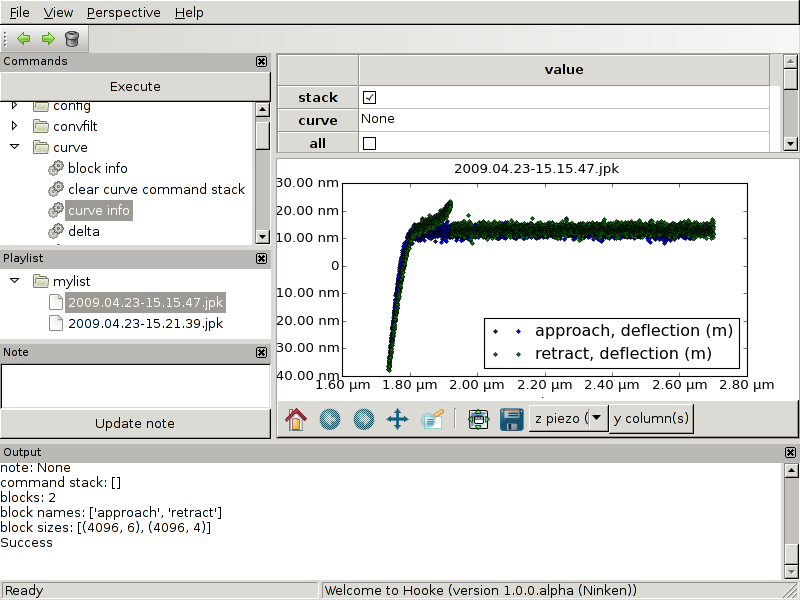
\includegraphics[width=\textwidth]{figures/binary/hooke-gui}
    \caption{Creating a playlist with two JPK files in the graphical
      Hooke interface.  You can see the output of the last \gui{curve
        info} call, which matches the output from the command line
      version (\cref{fig:hooke:cli}).  This screenshot is a bit
      cramped (to fit on a printed page), but the
      \href{http://www.wxwidgets.org}{wxWidgets} GUI toolkit provides
      automatic support for interactively rearranging and resizing
      panels.  The tree of commands is in the upper left corner.
      After you select a command, the table of argument in the upper
      right corner is populated with default values, which you can
      adjust as you see fit.  The \gui{Playlist} panel provides an
      easier interface for navigating to different playlists and
      curves than the using \gui{jump to playlist} and \gui{jump to
        curve} commands.\label{fig:hooke:gui}}
  \end{center}
\end{figure}

\section{Conclusions}
\label{sec:calibcant:conclusions}

Thermal cantilever calibration has been common practice for many years
now\citep{hutter93,florin95}, starting with estimates of thermal
noise\citep{martin87}.  However, discussion and explicit derivations
have been limited.  While this is likely done because the underlying
theory is ``obvious'', it makes it more likely that corner cases slip
by the notice of calibration experts\citep{hutter93-erratum} or
incorrect formul\ae\ are used during the fitting
(\cref{sec:calibcant:lorentzian}).  By centralizing calibration
procedures in an open package, \calibcant\ should both reduce the
effort needed to calibrate AFM cantilevers, improve the quality of the
calibration, and ease data sharing and archival.

